\documentclass[11pt,a4paper]{article}
\usepackage[utf8]{inputenc}
\usepackage[T1]{fontenc}
\usepackage[brazilian]{babel}
\usepackage{graphicx,booktabs,float}
\usepackage[a4paper,margin=2.5cm]{geometry}
\usepackage[hidelinks]{hyperref}
\title{O tempo de resolução de chamados de serviço público é previsível já na abertura? Evidências do serviço 311 de Nova York (2025)}
\author{Daniel de Carvalho Vianna\\ Departamento de Engenharia de Produção, Universidade de Brasília (UnB)}
\date{11/11/2026}
\begin{document}
\maketitle

\begin{abstract}
Este trabalho investiga se o tempo de resolução de chamados de serviço público pode ser previsto no momento da abertura, usando 3.655.042 chamados abertos em 2025 no serviço 311 de Nova York, obtidos como dados abertos. Os dados foram coletados por API, processados em PySpark e persistidos no BigQuery. 16,0\% dos chamados fechados levaram mais de 7 dias; um modelo de gradient boosting com variáveis conhecidas na abertura atingiu ROC-AUC de 0,962 em teste temporal, contra 0,954 de uma regra simples por tipo de demanda, e a correlação entre fila e tempo foi de 0,12 (mediana do valor absoluto, por agência). Segundo o critério declarado, a hipótese é CONFIRMADA.
\end{abstract}

\section{Introdução}
Serviços públicos urbanos operam como sistemas de filas: chamados chegam, aguardam e são atendidos por equipes de capacidade limitada. Prazo de atendimento, fila e cumprimento de prazos são medidas centrais na gestão de operações. Se o prazo de cada chamado puder ser antecipado na abertura, a organização pode informar prazos realistas, priorizar o acompanhamento de casos de risco e dimensionar capacidade. Este trabalho testa, com dados reais do serviço 311 de Nova York \cite{nyc311}, a hipótese de que o tempo de resolução é determinado principalmente pela natureza do chamado, conhecida na abertura, e pouco pela carga de trabalho do dia.

\section{Revisão da literatura}
A Lei de Little \cite{little} relaciona o número médio de itens em um sistema (L), a taxa média de chegada ($\lambda$) e o tempo médio de permanência (W) por L = $\lambda$W, e é um resultado básico da análise de filas e de fluxo em operações \cite{hopp}. Aplicada a um serviço de atendimento, sugere que, com capacidade fixa, filas maiores tendem a vir acompanhadas de tempos de resolução maiores, o que motiva a pergunta sobre a relação entre fila e tempo. Para prever o tempo ou o atraso de cada item, métodos de aprendizado supervisionado como o gradient boosting \cite{friedman}, disponíveis em bibliotecas como a scikit-learn \cite{sklearn}, são amplamente usados com dados tabulares que misturam variáveis categóricas e numéricas. Os registros de chamados 311 da cidade de Nova York \cite{nyc311}, publicados como dados abertos, permitem examinar essas ideias com dados reais. Este trabalho não propõe um método novo: aplica essa combinação de análise de fluxo e modelo preditivo a um ano de chamados, com validação temporal.

\section{Método}
\subsection{Dados e coleta}
Foram coletados, pela API SODA do NYC Open Data \cite{nyc311}, os chamados abertos entre 01/01/2025 e 31/12/2025, em páginas mensais de 50.000 linhas em CSV, sem token de aplicativo, com retentativas com espera exponencial e retomada. Foram obtidas 3.655.042 linhas (727,2 MB) entre 2026-11-11 21:39:36 e 2026-11-11 22:01:13 (UTC), conferidas mês a mês contra o total informado pela API. Foram usadas apenas colunas sem identificação de pessoas (agência, tipo de demanda, bairro, CEP, canal, status e datas). Os dados são públicos.

\subsection{Pipeline e regras de negócio}
O pipeline foi executado em um notebook do Google Colab, com ETL em PySpark local (arquitetura medalhão: raw, bronze, silver, gold) e persistência das camadas silver e gold no BigQuery Sandbox, com conferência das contagens de linhas. O modelo gold é uma estrela com a tabela fato fato\_chamado (grão: um chamado) e as tabelas dim\_data, dim\_agencia, dim\_tipo, dim\_local e agg\_agencia\_dia (carga por agência e dia). Regras: datas convertidas com TRY\_CAST; deduplicação por unique\_key; resolução em horas = fechamento - abertura; atraso = resolução acima de 168 horas (7 dias); resoluções negativas e chamados ainda abertos excluídos das análises de tempo. A fila no início do dia usa apenas chamados do recorte que foram fechados depois. O modelo usa somente variáveis conhecidas na abertura (agência, tipo, descritor, local, canal, hora, dia da semana, mês e chamados da agência nos 7 dias anteriores), com treino até 30/09 e teste de 01/10 a 31/12; o limiar de decisão é escolhido em um período de validação, e a importância das variáveis é medida por permutação. São comparados o gradient boosting \cite{friedman}, uma regressão logística e uma regra simples de taxa de atraso por tipo de demanda.

\subsection{Critério de avaliação da hipótese}
Definiu-se, antes da execução, que a hipótese é confirmada se (C1) o ROC-AUC do modelo no teste temporal for maior ou igual a 0,80 e (C2) a mediana do valor absoluto da correlação de Spearman entre a fila da agência e o tempo de resolução (uma correlação por agência) for menor que 0,30; parcialmente confirmada se apenas um critério for atendido; refutada se nenhum for.

\section{Resultados}
\subsection{Volume mensal e atrasos (P1)}
Foram abertos 3.655.042 chamados em 2025 (média de 10.014 por dia). O mês de maior volume foi janeiro (348.180) e o de menor volume foi fevereiro (255.364). Na data da coleta, 98,5\% dos chamados já estavam fechados. Entre os 3.600.109 chamados fechados com tempo de resolução válido, 16,0\% levaram mais de 7 dias, com variação mensal de 14,2\% (janeiro) a 19,1\% (julho). O tempo mediano de resolução foi de 6,6 h (0,3 dias) e o p90, de 411 h (17,1 dias). Foram excluídos das análises de tempo 54.933 chamados (1,5\%): os ainda abertos e os com fechamento anterior à abertura.
\begin{figure}[ht]
\centering
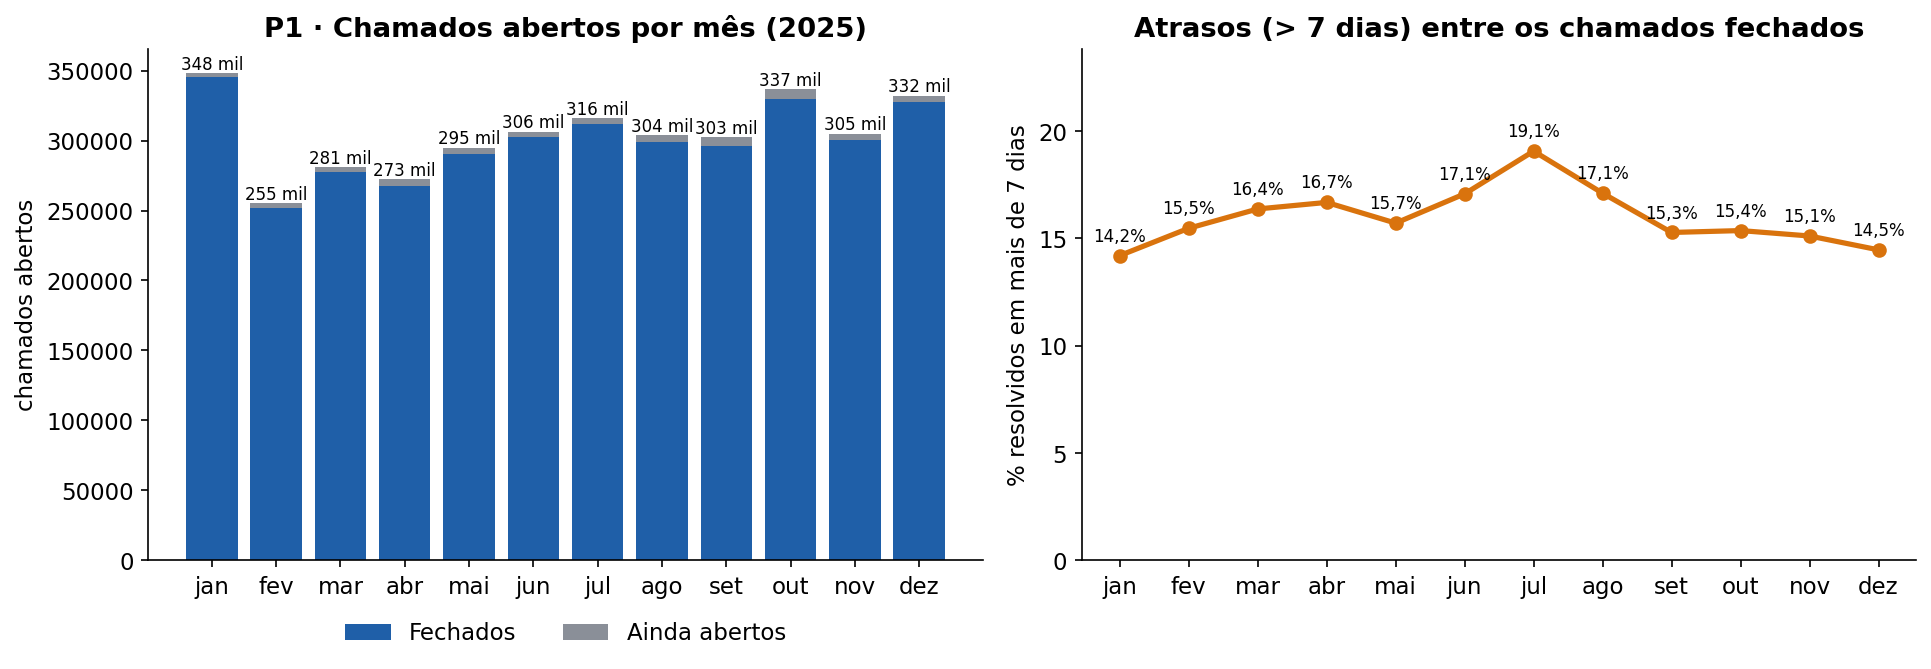
\includegraphics[width=0.85\linewidth]{p1.png}
\caption{Chamados abertos por mês e percentual resolvido em mais de 7 dias.}
\label{fig:p1}
\end{figure}
\subsection{Agências e tipos de demanda (P2)}
As três agências com mais chamados fechados são: NYPD (47,7\% dos chamados, mediana de 1,3 h, 0,0\% acima de 7 dias); HPD (21,4\% dos chamados, mediana de 79,2 h, 35,3\% acima de 7 dias); DSNY (9,0\% dos chamados, mediana de 32,7 h, 10,7\% acima de 7 dias). Entre as agências com pelo menos 1.000 chamados, a taxa de atraso varia de 0,0\% a 100,0\%. Os atrasos são concentrados: três agências respondem por 67,1\% dos 574.329 chamados resolvidos em mais de 7 dias e os dez tipos de demanda com mais atrasos respondem por 49,6\%. Os tipos que mais geram atrasos são: UNSANITARY CONDITION (74.021 atrasos, 63,0\% dos seus chamados); PLUMBING (37.096 atrasos, 53,5\% dos seus chamados); PAINT/PLASTER (30.220 atrasos, 51,1\% dos seus chamados).
\begin{table}[ht]
\centering\small
\begin{tabular}{lrrrr}
\toprule
Agência & Chamados & Mediana (h) & p90 (h) & \% > 7 dias \\
\midrule
NYPD & 1.717.526 & 1,3 & 7 & 0,0\% \\
HPD & 771.454 & 79,2 & 956 & 35,3\% \\
DSNY & 323.604 & 32,7 & 174 & 10,7\% \\
DOT & 206.250 & 46,3 & 421 & 27,3\% \\
DEP & 194.715 & 21,6 & 174 & 11,9\% \\
DOB & 103.068 & 278,2 & 4.446 & 55,1\% \\
\bottomrule
\end{tabular}
\caption{Agências com mais chamados fechados.}
\label{tab:ag}
\end{table}
\begin{figure}[ht]
\centering
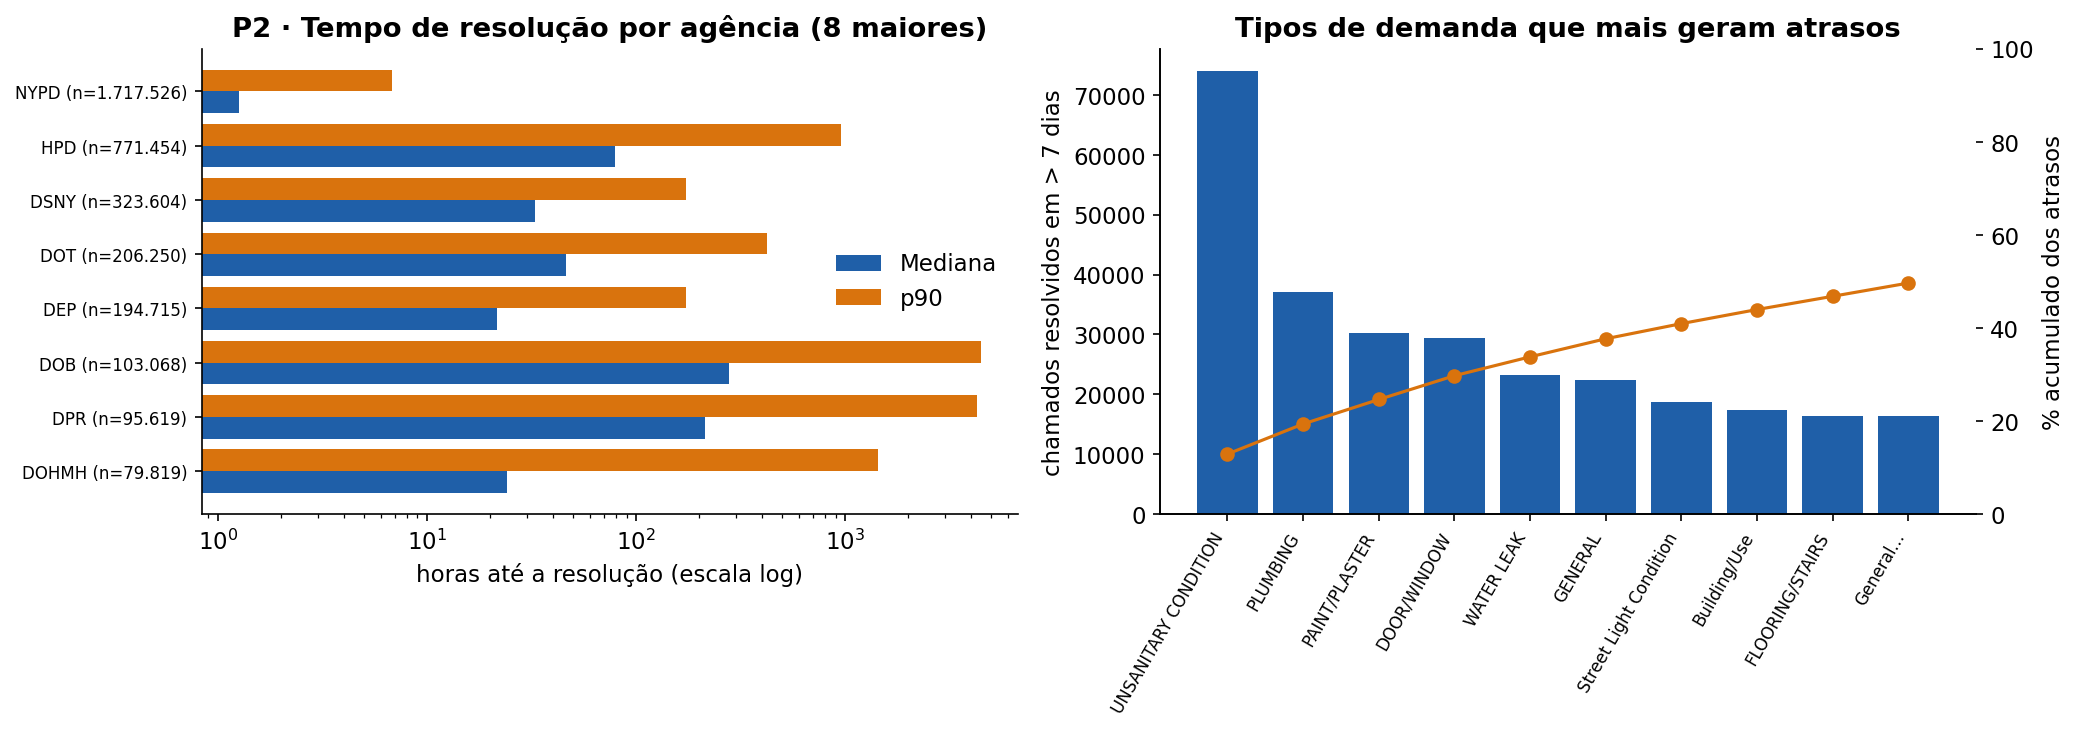
\includegraphics[width=0.85\linewidth]{p2.png}
\caption{Tempo de resolução por agência e tipos de demanda que mais geram atrasos.}
\label{fig:p2}
\end{figure}
\subsection{Momento da abertura (P3)}
A taxa de atraso (> 7 dias) varia 7,7 pontos percentuais entre os dias da semana de abertura (maior em segunda-feira, 18,4\%; menor em domingo, 10,7\%), 4,9 p.p. entre os meses e 16,4 p.p. entre as horas do dia (considerando horas com ao menos 1.000 chamados). Para comparação, a diferença entre as agências é de 100,0 p.p., 6,1 vezes a maior variação temporal. Cautela: 0,1\% das aberturas estão registradas exatamente à meia-noite, o que indica registros sem hora e limita a leitura da hora de abertura.
\begin{figure}[ht]
\centering
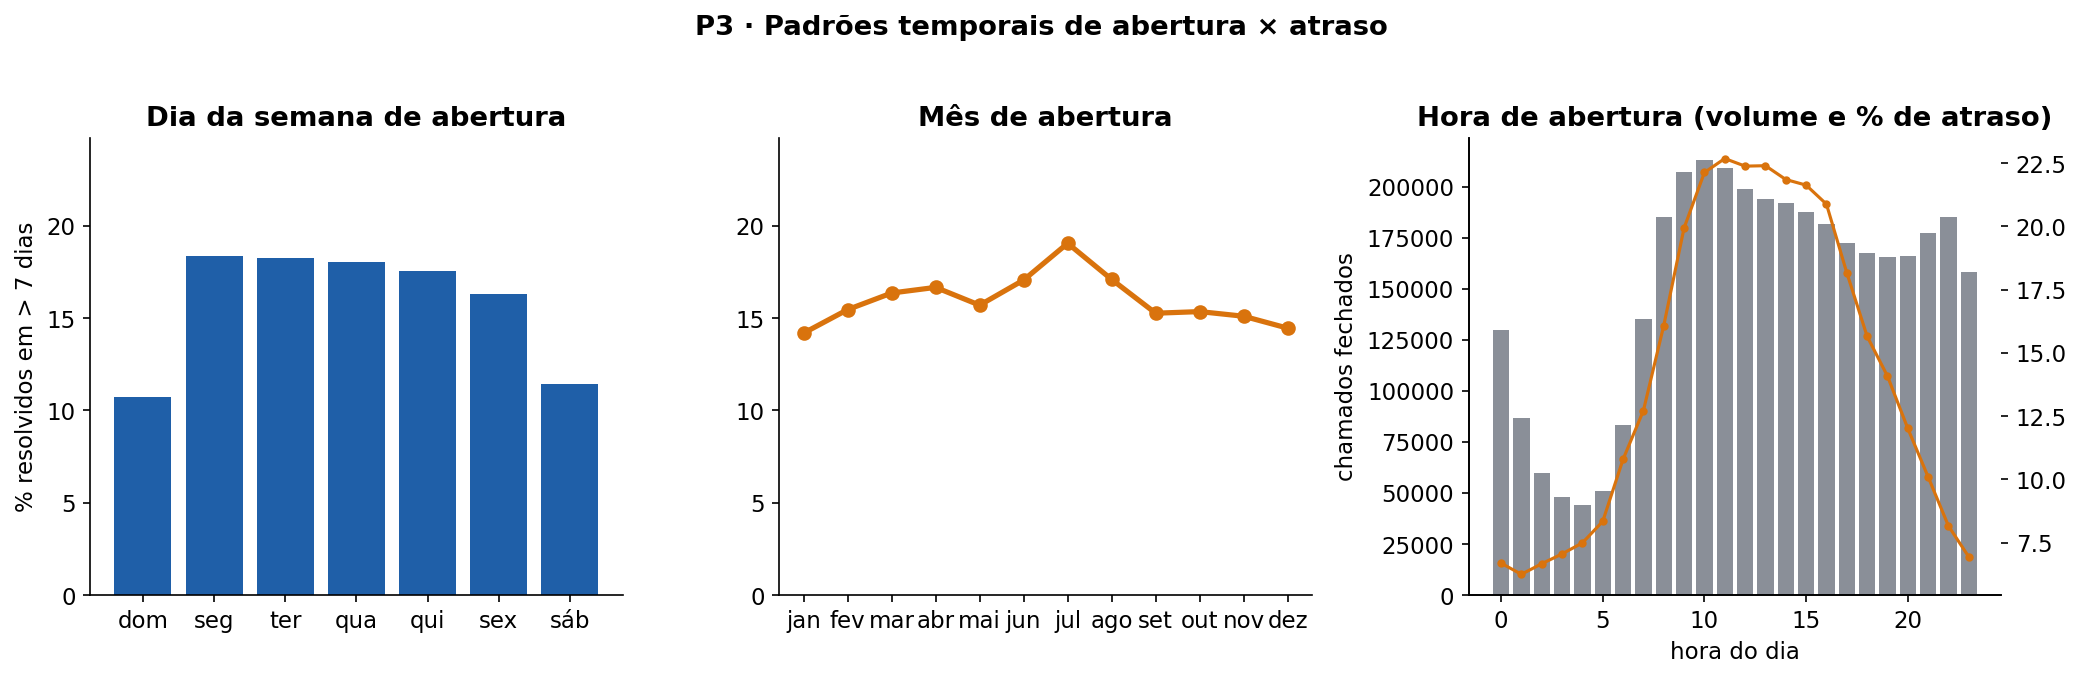
\includegraphics[width=0.85\linewidth]{p3.png}
\caption{Atrasos segundo dia da semana, mês e hora de abertura.}
\label{fig:p3}
\end{figure}
\subsection{Carga de trabalho e tempo de resolução (P4)}
Em 12 agências com ao menos 60 dias válidos (cada dia com no mínimo 30 chamados fechados), a correlação de Spearman entre a fila no início do dia e a mediana do tempo de resolução dos chamados abertos naquele dia tem mediana 0,09 (associação praticamente nula) e mediana do valor absoluto 0,12; 33\% das agências têm |$\rho$| $\geq$ 0,30. Usando os chamados criados nos 7 dias anteriores como medida de carga, a mediana do |$\rho$| é 0,13. Pela Lei de Little (L = $\lambda$W), com capacidade fixa uma fila maior tenderia a vir acompanhada de tempos maiores; a magnitude observada indica quanto disso aparece nos dados. Cautela: a fila usa só chamados abertos em 2025 que foram fechados depois e começa subestimada em janeiro (por isso o período de análise começa em fevereiro), e correlação não implica causalidade.
\begin{figure}[ht]
\centering
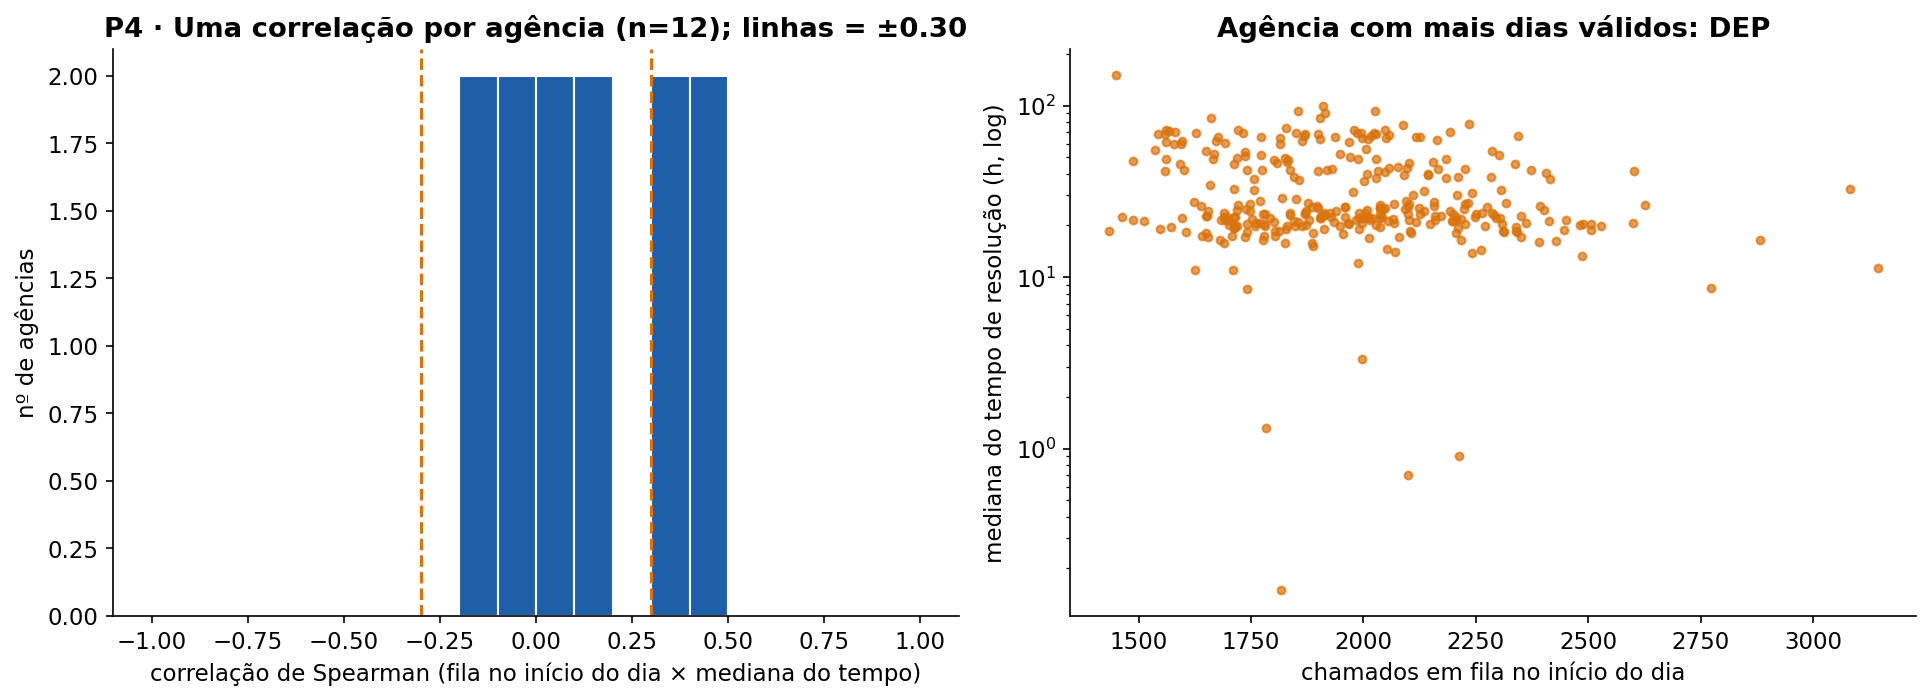
\includegraphics[width=0.85\linewidth]{p4.png}
\caption{Correlação entre fila e tempo de resolução, por agência.}
\label{fig:p4}
\end{figure}
\subsection{Modelo preditivo (P5)}
Com validação temporal (treino: 293.481 chamados abertos até 30/09; teste: 106.287 abertos de 01/10 a 31/12; prevalência de atraso de 16,4\% no treino e 15,0\% no teste), o ROC-AUC no teste foi de 0,962 para o gradient boosting, 0,960 para a regressão logística e 0,954 para a regra simples de taxa de atraso por tipo de demanda (aleatório = 0,500). O ganho do modelo sobre a regra por tipo é de 0,007 em AUC. No limiar escolhido na validação (0,41), o modelo atinge precisão de 67,8\%, revocação de 83,9\% e F1 de 0,75. No decil de maior risco, 75,2\% dos chamados de fato atrasam (contra 15,0\% na média), e esse decil captura 50,2\% de todos os atrasos. As variáveis de maior importância por permutação (queda do AUC) são: tipo de demanda (0,162), descritor (0,022), carga: chamados da agência nos 7 dias anteriores (0,013). A carga de trabalho (chamados da agência nos 7 dias anteriores) tem queda de AUC de 0,013. O modelo usa uma amostra de 399.768 chamados (11\% da base de tempo).
\begin{table}[ht]
\centering\small
\begin{tabular}{lrrr}
\toprule
Modelo & ROC-AUC & AP & Precisão no decil \\
\midrule
Gradient boosting & 0,962 & 0,774 & 75,2\% \\
Regressão logística & 0,960 & 0,767 & 74,7\% \\
Regra por tipo de demanda & 0,954 & 0,734 & 71,9\% \\
\bottomrule
\end{tabular}
\caption{Desempenho no teste temporal (out–dez).}
\label{tab:mod}
\end{table}
\begin{figure}[ht]
\centering
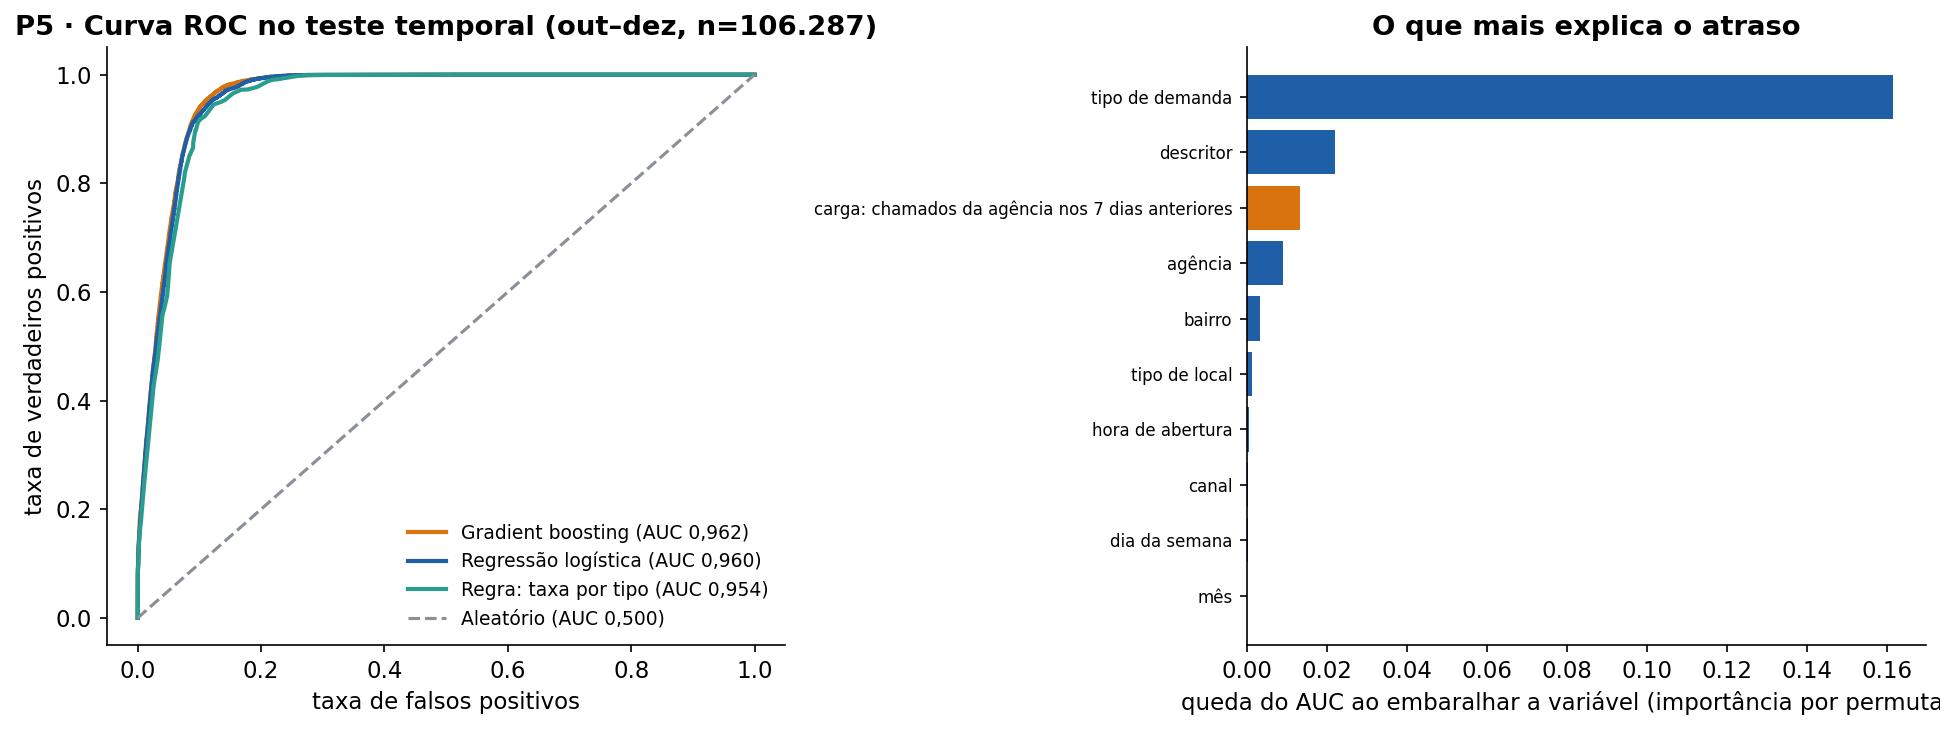
\includegraphics[width=0.85\linewidth]{p5.png}
\caption{Curvas ROC no teste temporal e importância das variáveis.}
\label{fig:p5}
\end{figure}

\section{Discussão}
Critério declarado antes da execução: a hipótese é CONFIRMADA se (C1) o ROC-AUC do modelo no teste temporal for maior ou igual a 0,80 e (C2) a mediana do valor absoluto da correlação de Spearman entre a fila da agência e o tempo de resolução for menor que 0,30; PARCIALMENTE CONFIRMADA se apenas um dos dois critérios for atendido; REFUTADA se nenhum for. Resultado: C1: ROC-AUC no teste = 0,962 (atende $\geq$ 0,80); C2: mediana do |$\rho$| entre fila e tempo = 0,12 (atende < 0,30). Veredito: hipótese CONFIRMADA. O atraso é razoavelmente previsível já na abertura e a carga diária da agência explica pouco do tempo de resolução. Na prática, isso sustenta informar ao cidadão um prazo esperado por tipo de demanda e agência e concentrar o acompanhamento nos chamados classificados como de alto risco, em vez de tratar a carga do dia como a principal causa dos atrasos. Ressalvas: os dados são de uma única cidade e de um único ano; o fechamento é um registro administrativo (pode não coincidir com a solução real do problema); parte das horas de abertura e fechamento é registrada à meia-noite; o AUC mede a capacidade de ordenar chamados por risco, não a calibração das probabilidades; e os limiares (0,80 e 0,30) são uma escolha do autor, explicitada para que o resultado seja auditável.

\section{Qualidade dos dados e limitações}
A análise de qualidade cobriu completude, unicidade, conformidade, consistência, acurácia e atualidade; os resultados detalhados estão no repositório (README e figuras de qualidade).
\begin{itemize}
\item Uma única cidade e um único ano; os resultados podem não se generalizar.
\item O fechamento é um registro administrativo e pode não coincidir com a solução efetiva do problema.
\item 0,1\% das aberturas estão registradas à meia-noite (registros sem hora).
\item 1,5\% dos chamados seguiam abertos na coleta e foram excluídos das análises de tempo (censura à direita).
\item A fila considera apenas chamados de 2025 fechados depois, e o modelo foi avaliado em um único corte temporal.
\item Os limiares do critério de veredito (0,80 para o AUC e 0,30 para a correlação) são uma escolha do autor.
\end{itemize}

\section{Conclusão}
Nos dados de 2025, a hipótese de que o atraso é previsível na abertura e pouco dependente da carga do dia é CONFIRMADA, segundo o critério declarado. Como trabalhos futuros, sugerem-se a previsão do tempo de resolução (regressão ou análise de sobrevivência), a inclusão de variáveis de processo, clima e calendário, e a validação em mais de um período e em outras cidades.

\begin{thebibliography}{9}
\bibitem{nyc311} City of New York. \textit{311 Service Requests from 2010 to Present}. NYC Open Data, conjunto \texttt{erm2-nwe9}. \url{https://data.cityofnewyork.us/Social-Services/311-Service-Requests-from-2010-to-Present/erm2-nwe9}.
\bibitem{little} Little, J. D. C. A proof for the queuing formula: $L = \lambda W$. \textit{Operations Research}, 9(3), 383--387, 1961.
\bibitem{hopp} Hopp, W. J.; Spearman, M. L. \textit{Factory Physics}. 3rd ed. Waveland Press, 2008.
\bibitem{friedman} Friedman, J. H. Greedy function approximation: a gradient boosting machine. \textit{Annals of Statistics}, 29(5), 1189--1232, 2001.
\bibitem{sklearn} Pedregosa, F. et al. Scikit-learn: machine learning in Python. \textit{Journal of Machine Learning Research}, 12, 2825--2830, 2011.
\end{thebibliography}
\end{document}
